\documentclass[a4paper,journal]{IEEEtran}

\usepackage[utf8]{inputenc}
\usepackage[T1]{fontenc}
\usepackage{mathptmx}
\usepackage{textcomp}
\usepackage[UKenglish]{babel}
\usepackage{amsmath, amssymb}
\usepackage{float}
\usepackage{xcolor}
\definecolor{backcolor}{rgb}{0.95,0.95,0.92}
\definecolor{codegreen}{rgb}{0,0.6,0}
\definecolor{codepurple}{rgb}{0.58,0,0.82}
\usepackage{listings}
\lstdefinestyle{code}{
	backgroundcolor=\color{backcolor},
	commentstyle=\color{codegreen},
	keywordstyle=\color{magenta},
	stringstyle=\color{codepurple},
	frame=single,
	captionpos=b,
	showspaces=false,
	showstringspaces=false,
	breaklines=true,
}
\lstset{style=code}
\usepackage[hidelinks]{hyperref}
\hypersetup{
	colorlinks=false
}
\usepackage[style=ieee]{biblatex}
\bibliography{sources/biblio}
\renewcommand{\baselinestretch}{1.5}

\setlength{\parindent}{0pt}
\setlength{\parskip}{1em}

% figure support
\usepackage{import}
\usepackage{xifthen}
\pdfminorversion=7
\usepackage{pdfpages}
\usepackage{transparent}
\newcommand{\incfig}[1]{%
	\def\svgwidth{\columnwidth}
	\import{./figures/}{#1.pdf_tex}
}

\pdfsuppresswarningpagegroup=1


% correct bad hyphenation here
\hyphenation{op-tical net-works semi-conduc-tor}


\begin{document}
\title{Meng in Electronic \& Computer Engineering}
\author{Michael~Lenehan%
\thanks{Liam Meany, Department
of Electronic Engineering, Dublin City University, Dublin,
Ireland e-mail: liam.meany@dcu.ie.}% <-this % stops a space
\thanks{Dr. Martin Collier, Department
of Electroonic Engineering, Dublin City University, Dublin,
Ireland e-mail: martin.collier@dcu.ie.}% <-this % stops a space
}


% The paper headers
\markboth{MEng in Electronic \& Computer Engineering}%
{Shell \MakeLowercase{\textit{et al.}}: Bare Demo of IEEEtran.cls for IEEE Journals}

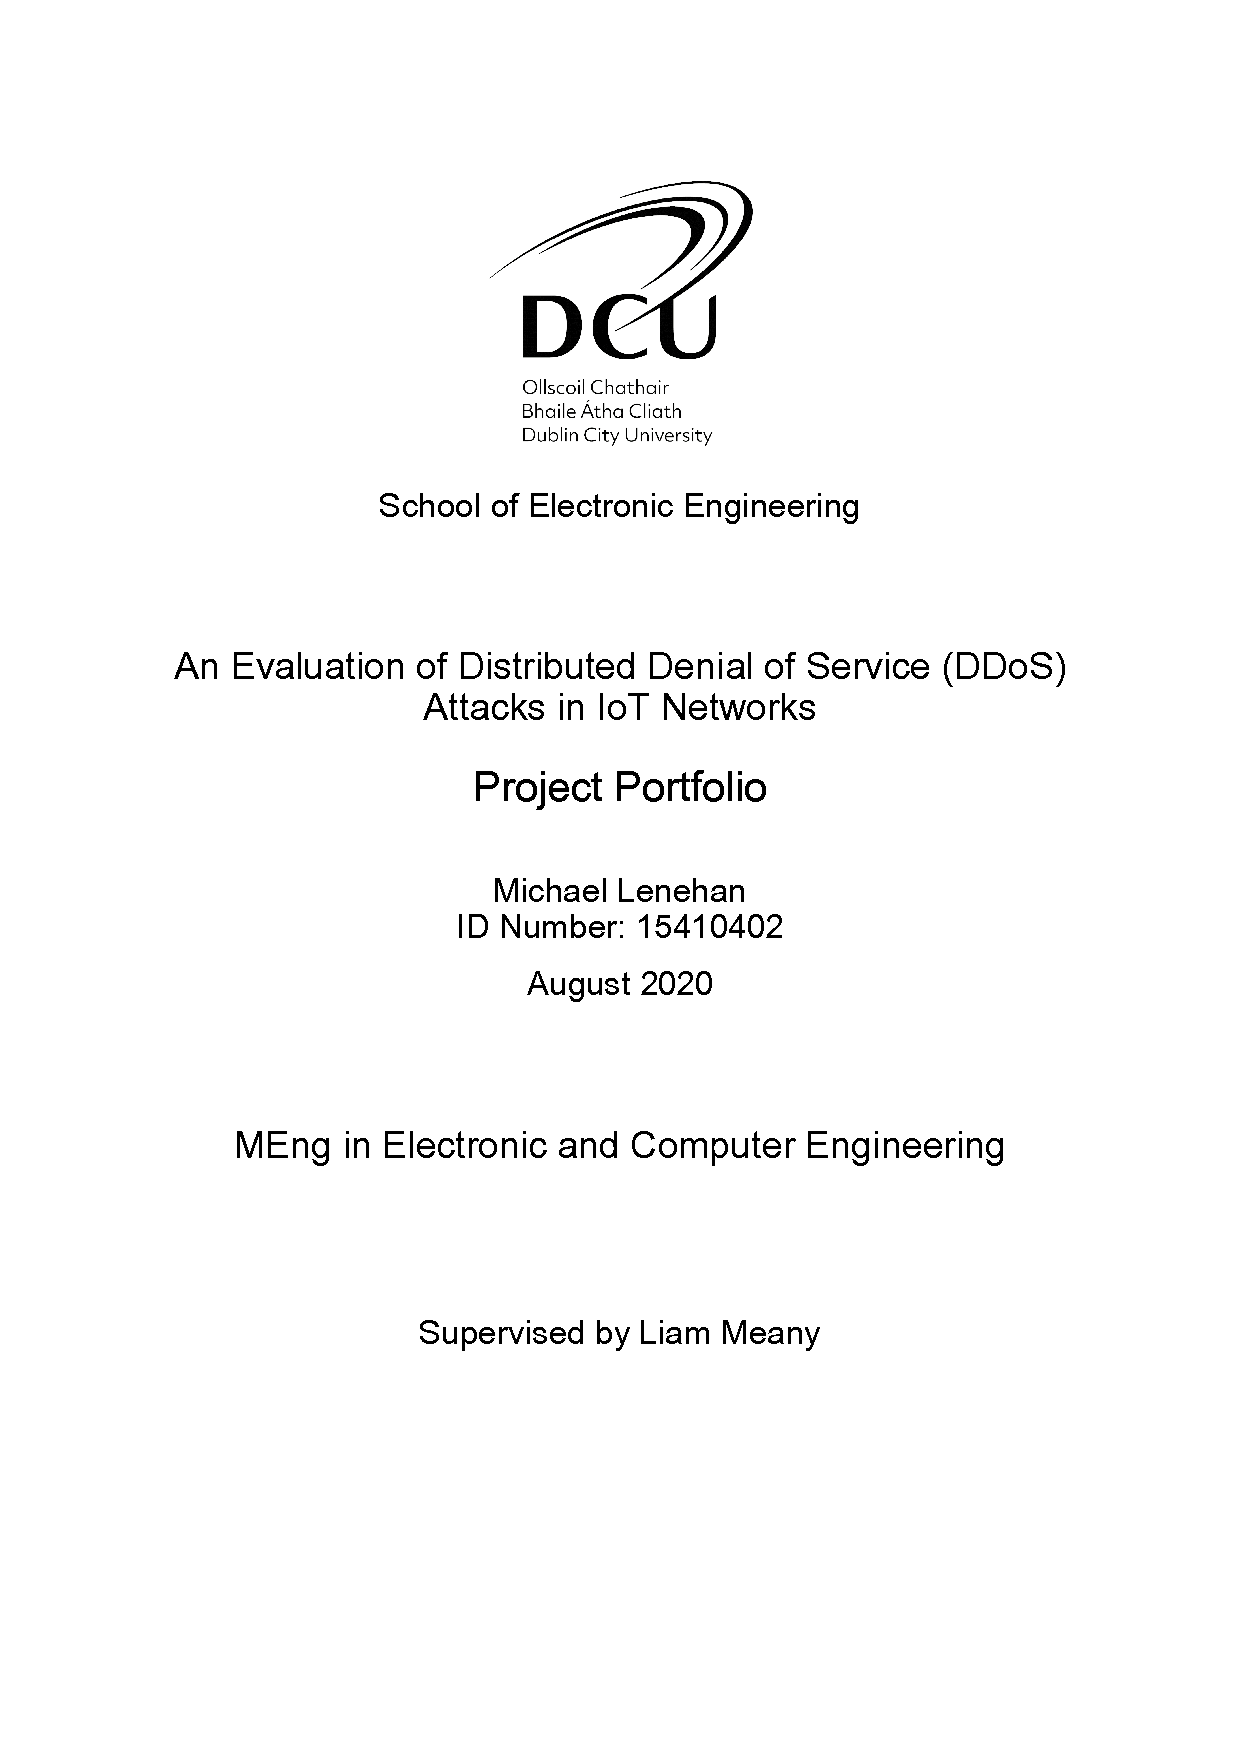
\includepdf{cover/coverpage}
\maketitle

\begin{abstract}
The abstract goes here.
\end{abstract}

% Note that keywords are not normally used for peerreview papers.
\begin{IEEEkeywords}
IEEE, IEEEtran, journal, \LaTeX, paper, template.
\end{IEEEkeywords}
\section{Introduction}
\IEEEPARstart{T}{his} demo file is intended to serve as a ``starter file''
for IEEE journal papers produced under \LaTeX\ using
IEEEtran.cls version 1.8b and later.
% You must have at least 2 lines in the paragraph with the drop letter
% (should never be an issue)
I wish you the best of success.

\hfill mds

\hfill August 31, 2020

\subsection{Subsection Heading Here}
Subsection text here.

% needed in second column of first page if using \IEEEpubid
%\IEEEpubidadjcol

\subsubsection{Subsubsection Heading Here}
Subsubsection text here.

\section{Conclusion}
The conclusion goes here.

\clearpage
\appendices
\section*{}
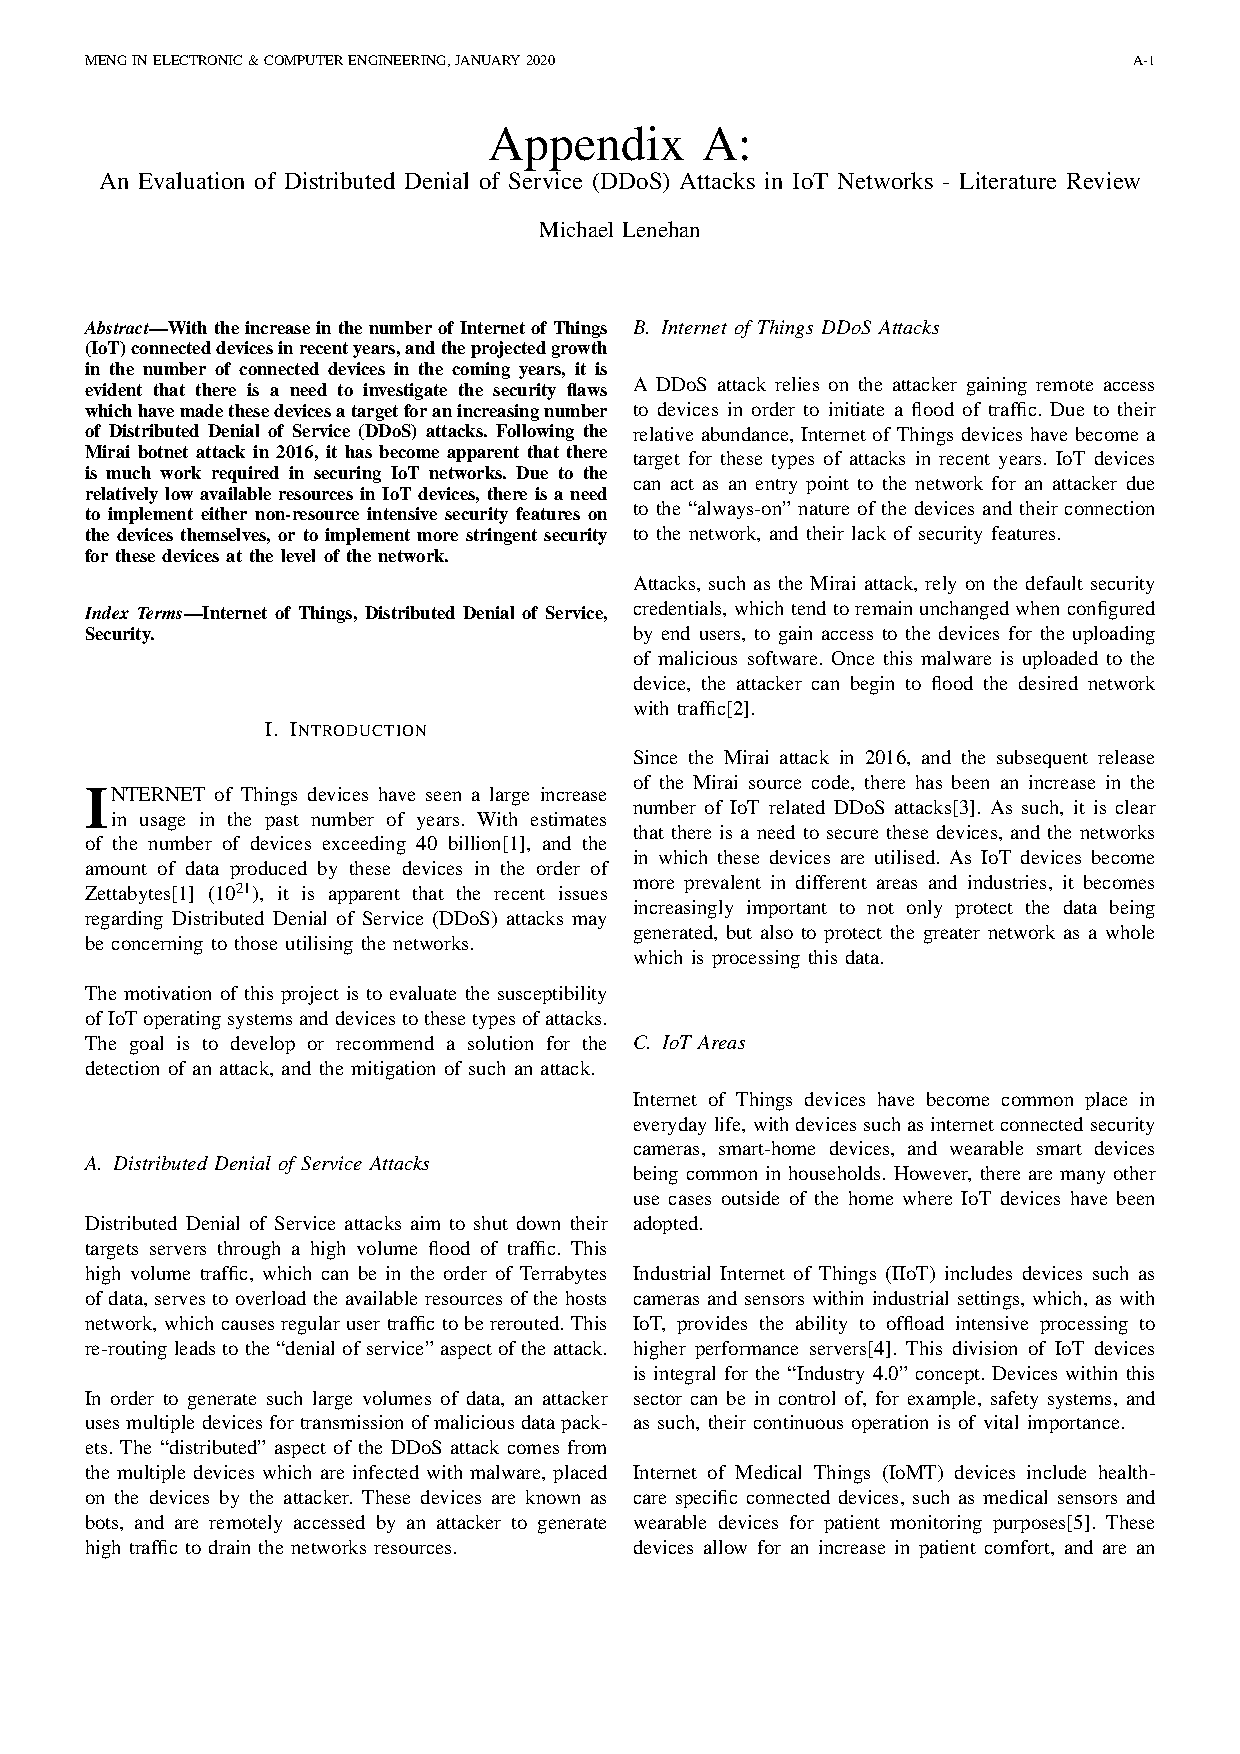
\includepdf[pages=-]{Portfolio/LitReview/LitReview}
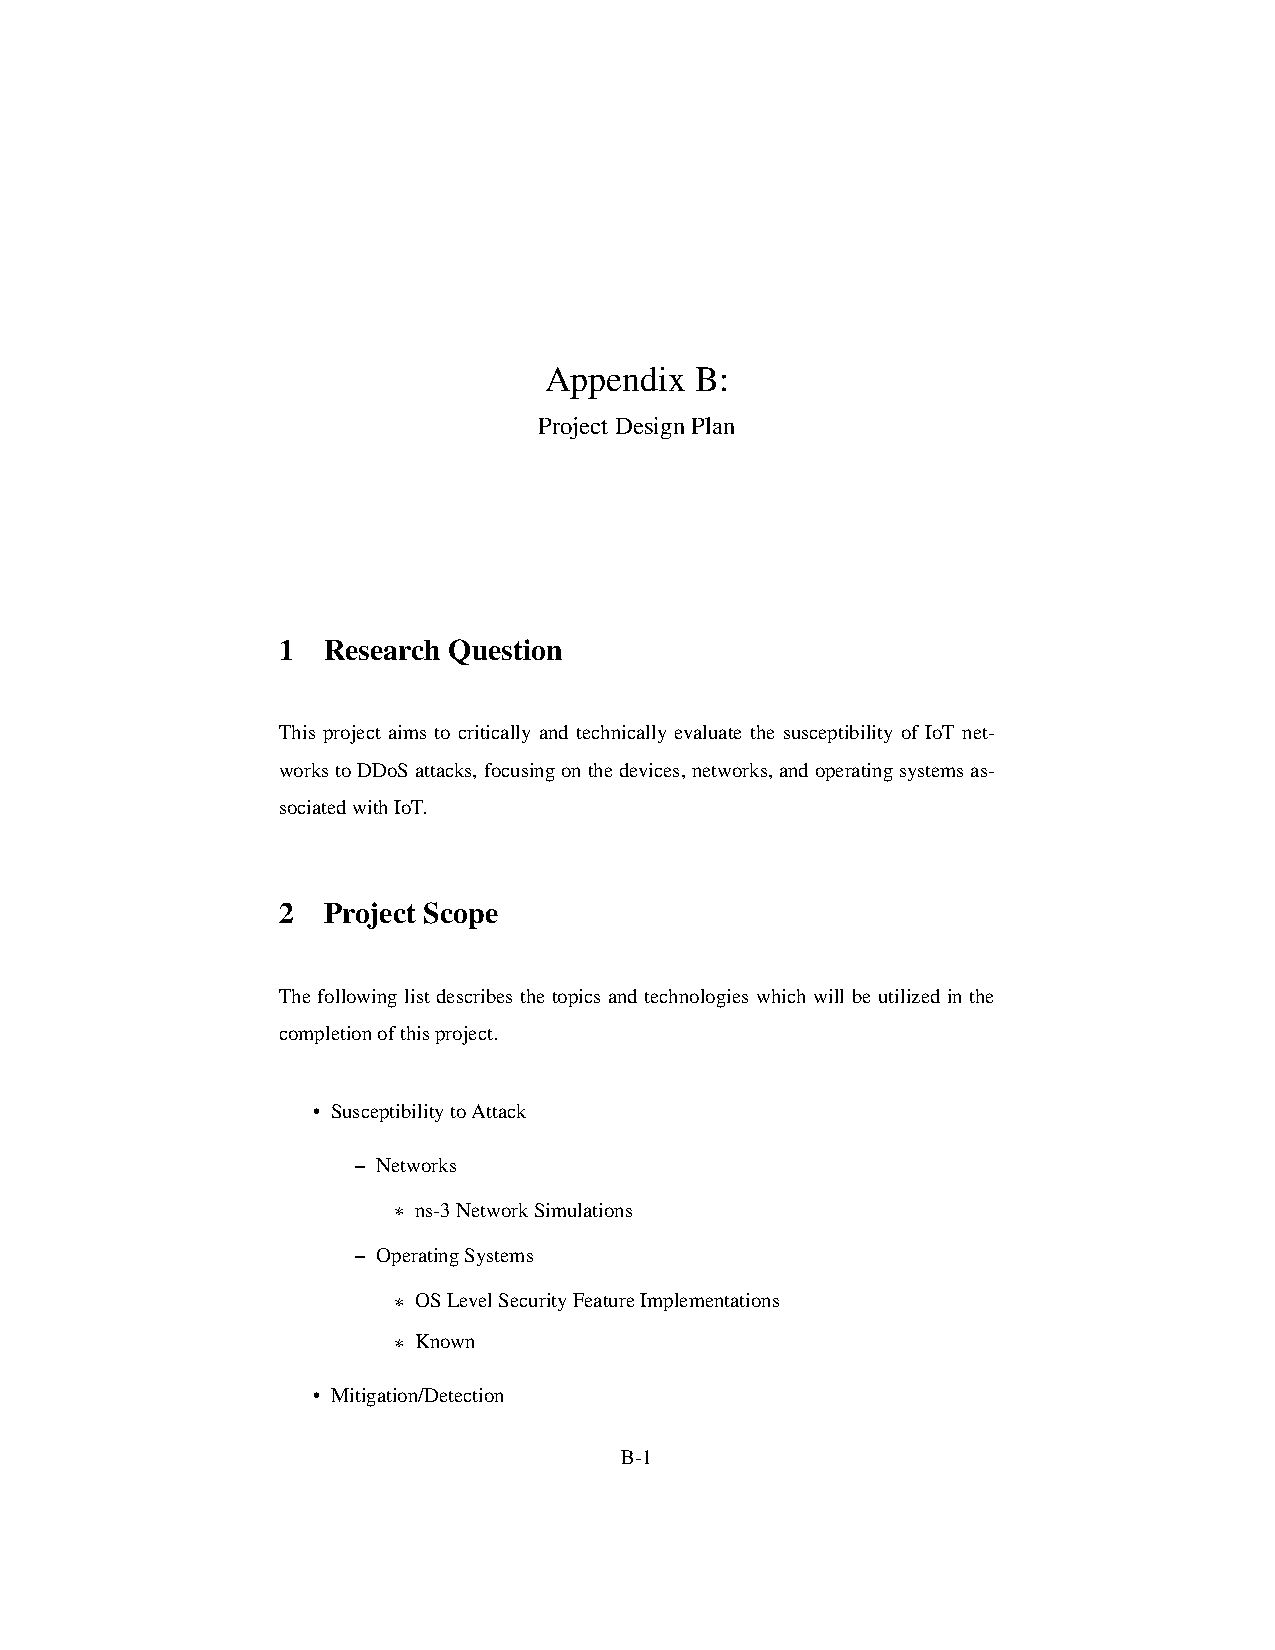
\includepdf[pages=-]{Portfolio/ProjectDesignPlan/designPlan}
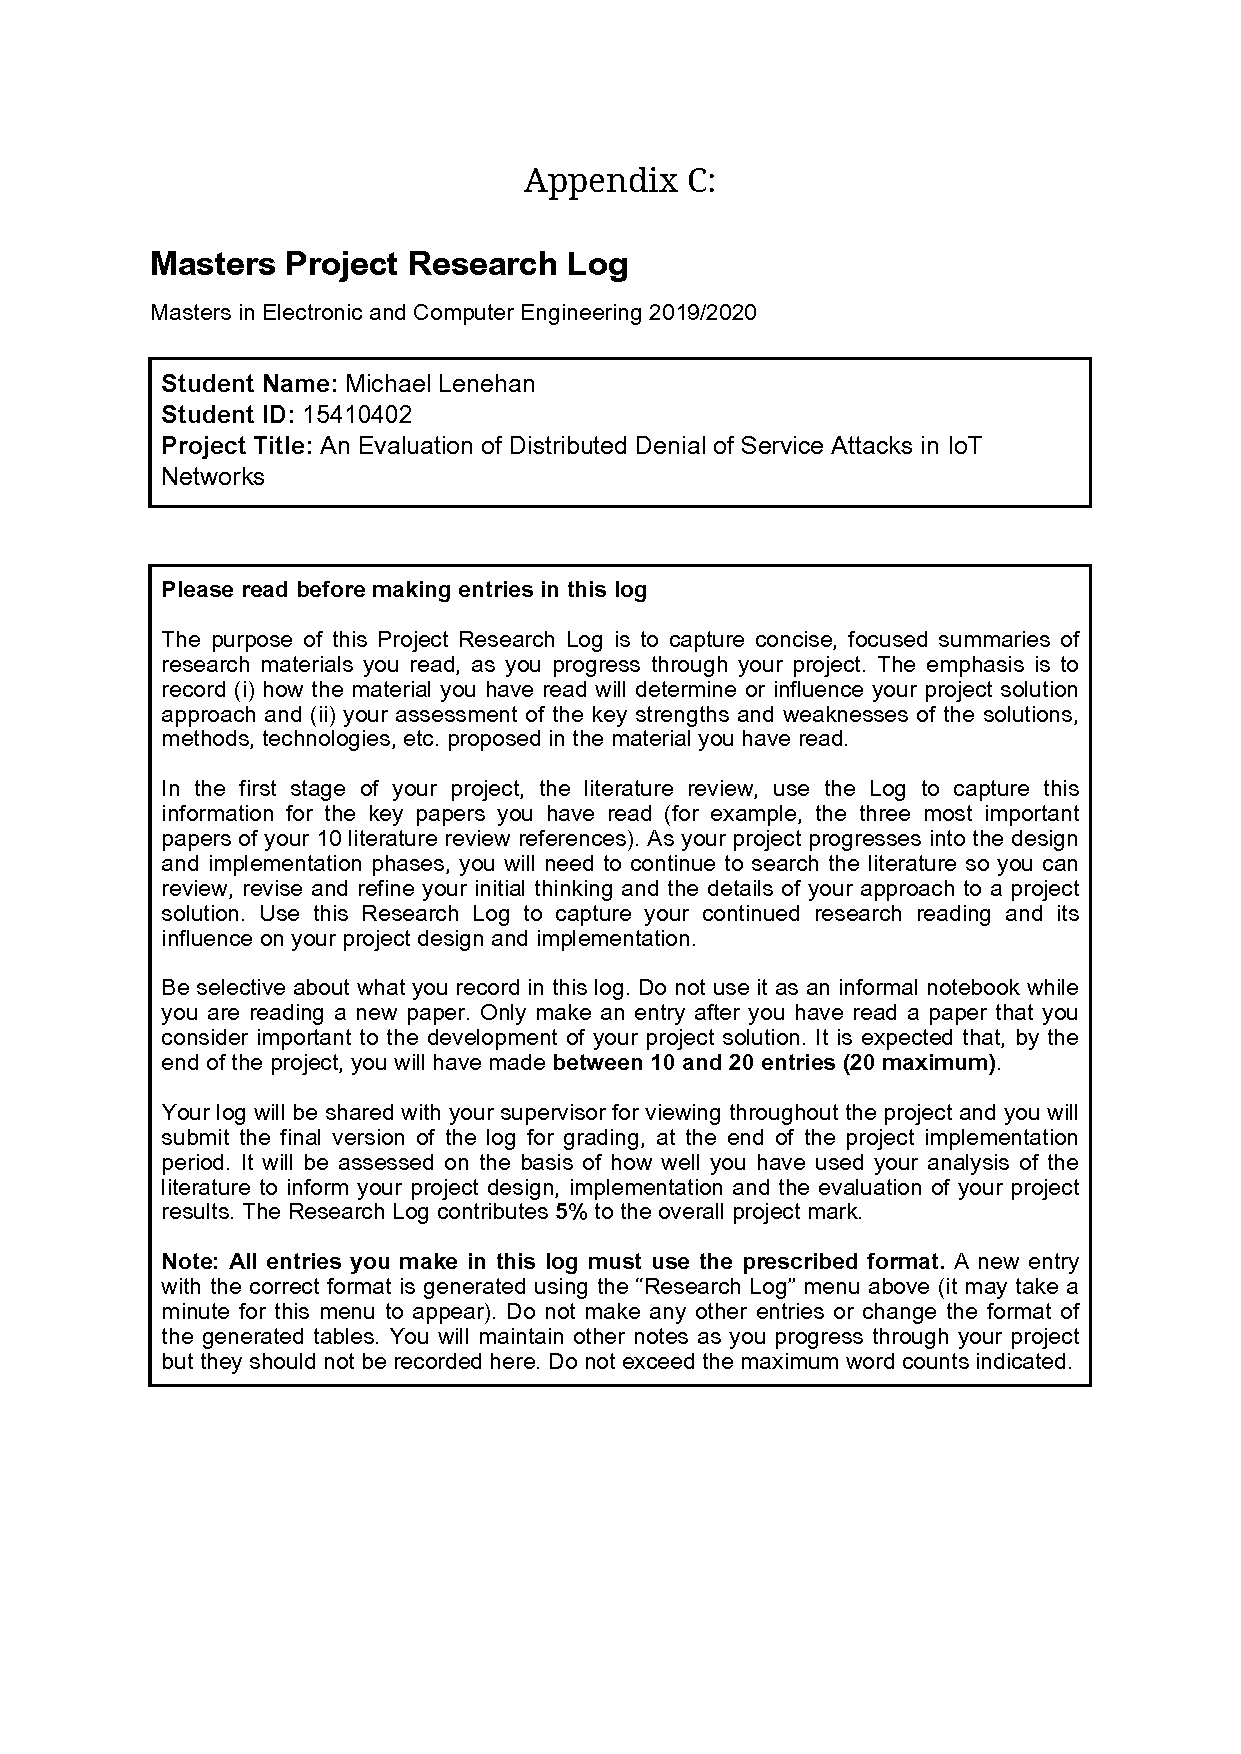
\includepdf[pages=-]{Portfolio/ResearchLog/researchLog}
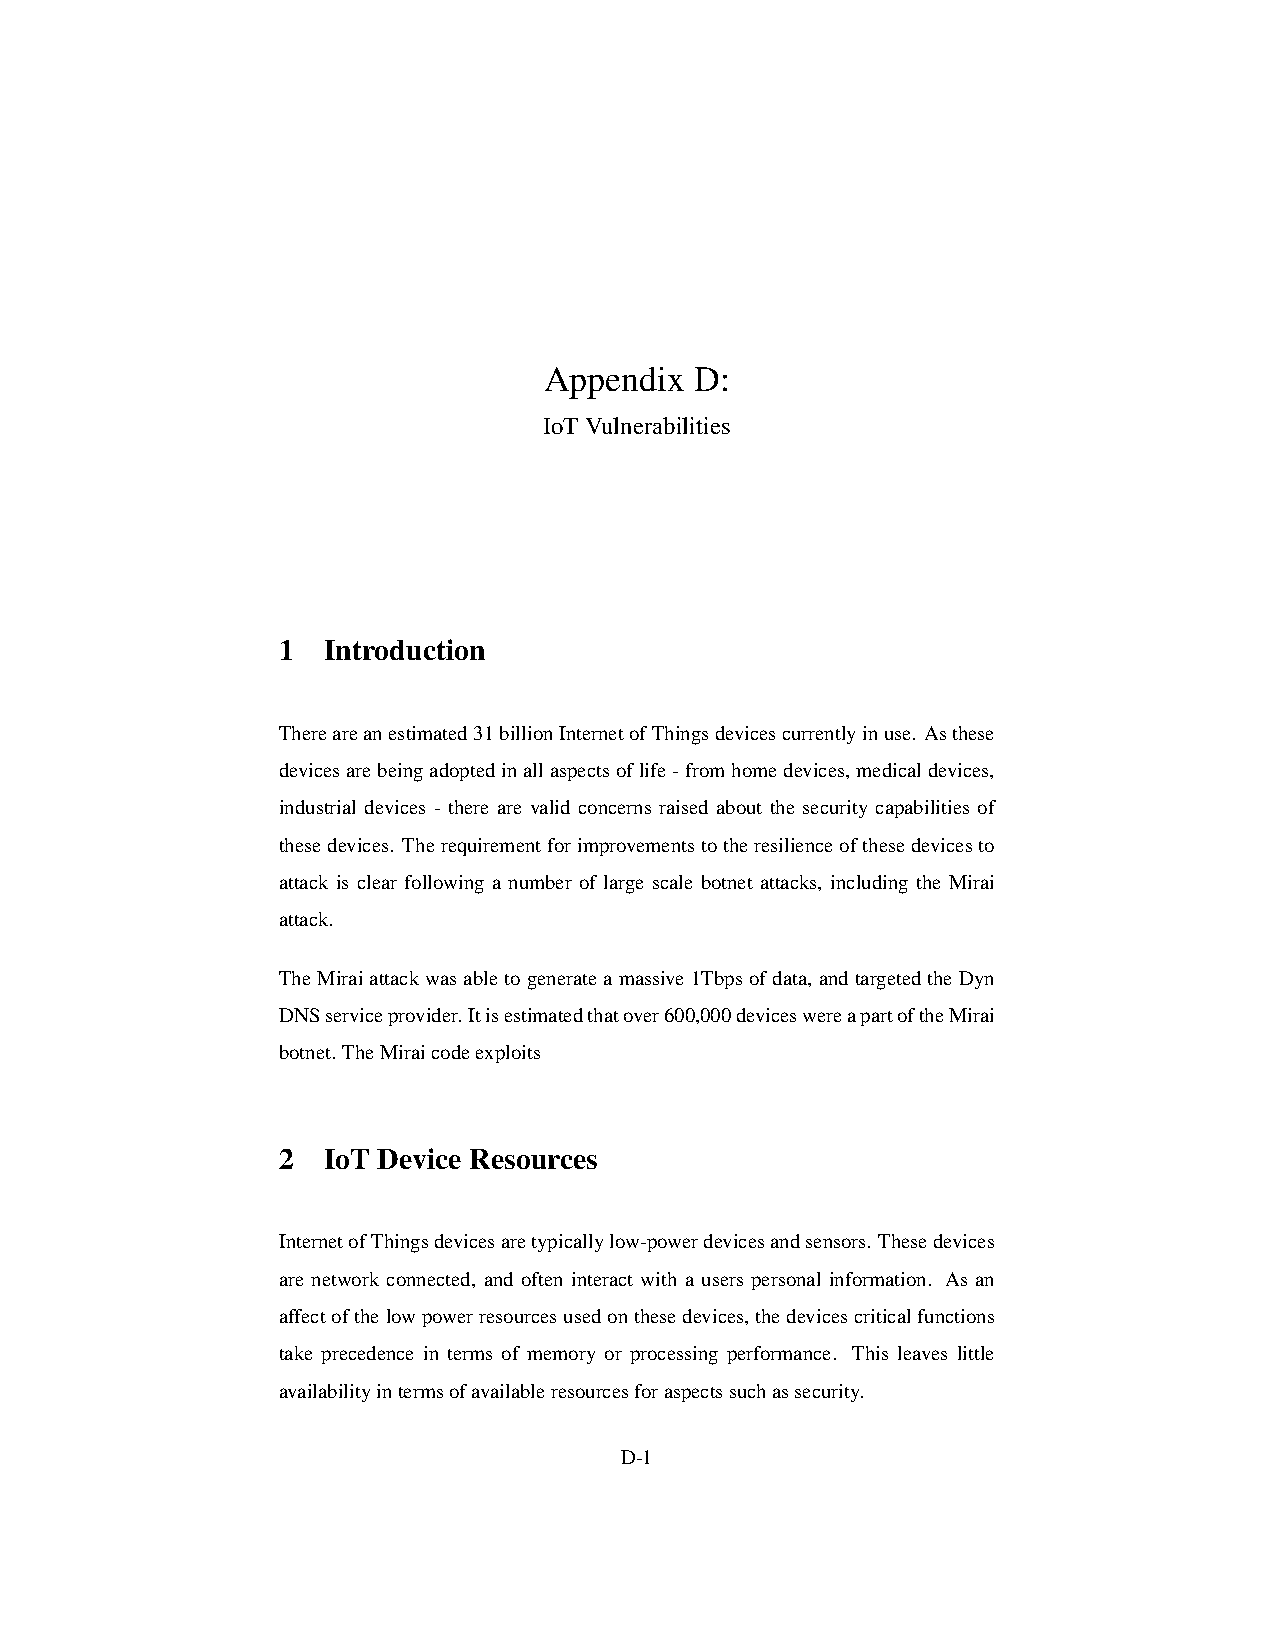
\includepdf[pages=-]{Portfolio/IoTVulnerabilities/IoTVulnerabilities}
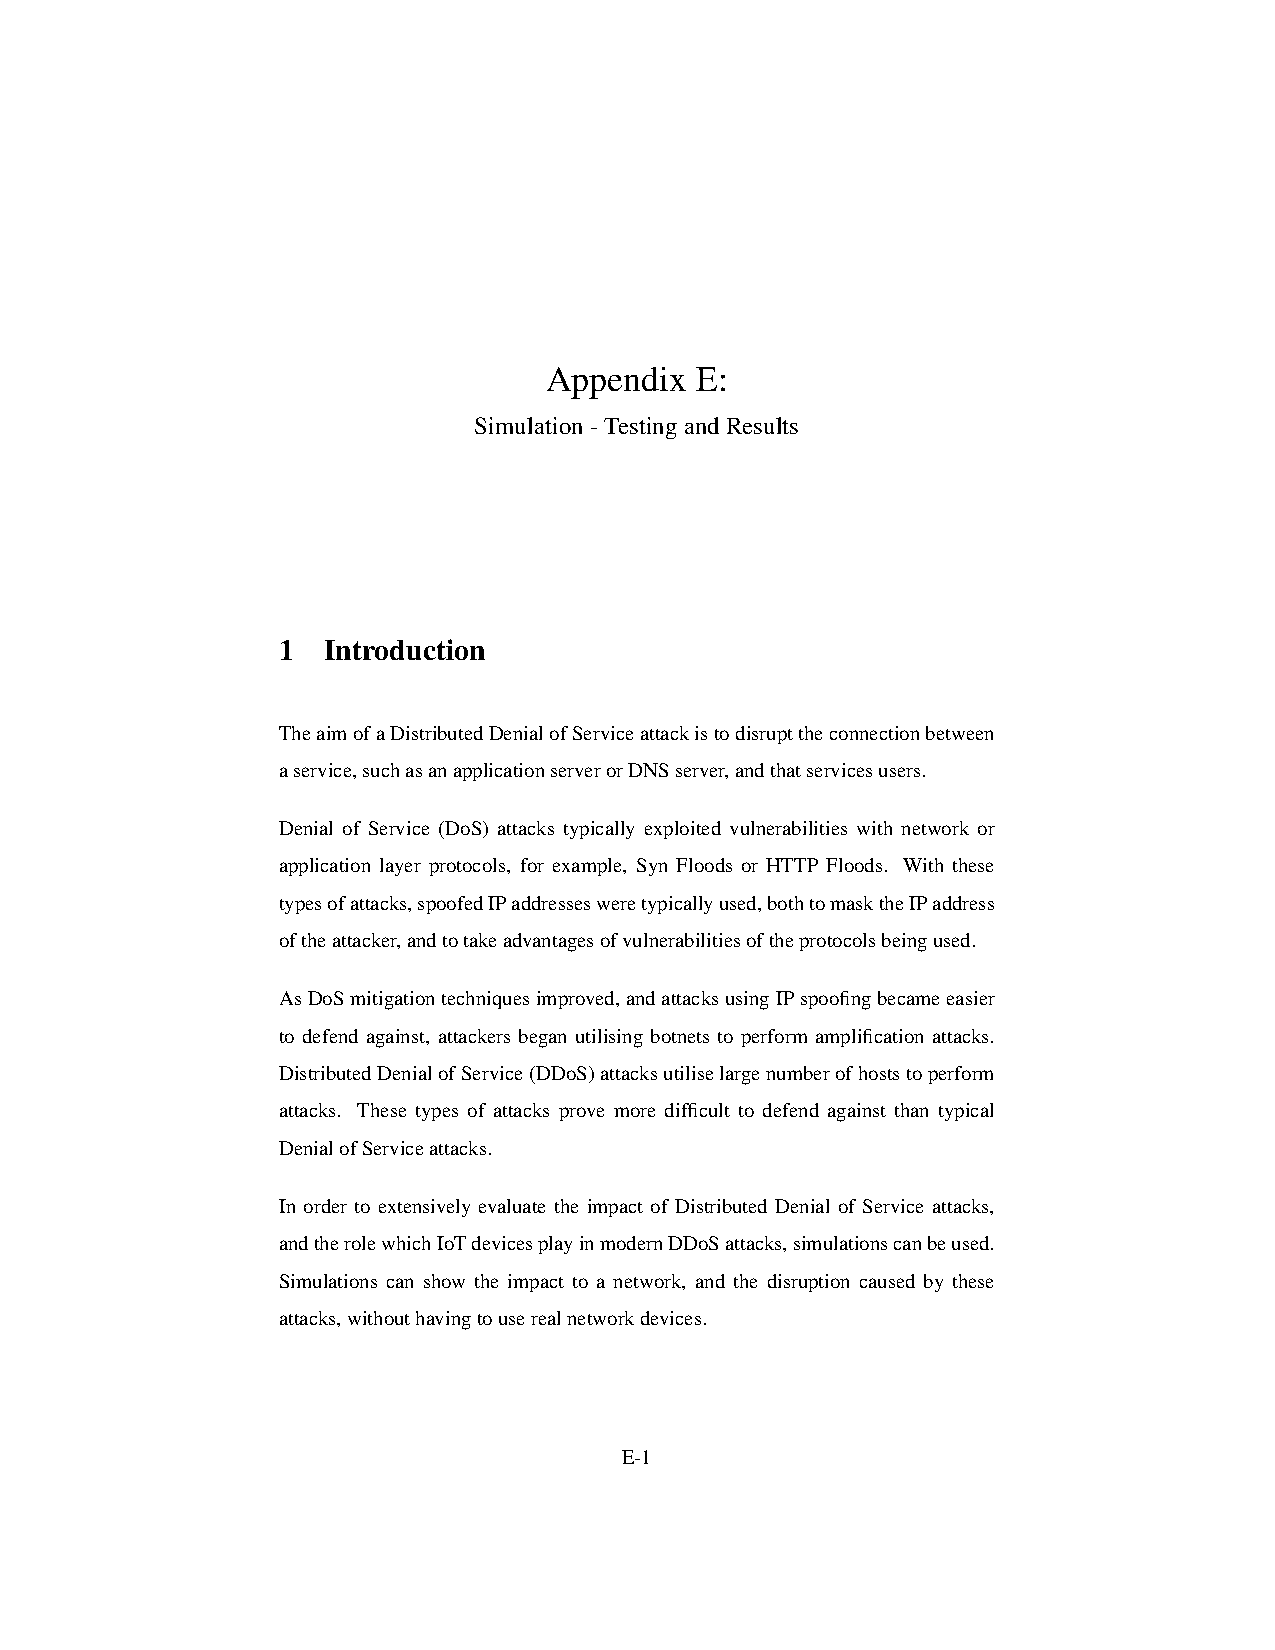
\includepdf[pages=-]{Portfolio/Simulation/Simulation}

\includepdf[pages=-]{Portfolio/Mitigation/Mitigation}
\printbibliography
\end{document}
